\chapter{Formal grammars and finite state automata}
\section{Formal grammars}
\lecture{2}{21/1}

Even though this topic has been approached several times
in other modules, we will redefine formal languages.

\begin{definition}[Strings and alphabets]
    A \textbf{word} (or \textbf{string}) is defined as a finite sequence
    of members of an underlying base set, called the
    \textbf{alphabet} of a word (or collection of words).
\end{definition}

\begin{remark}
    We can also construct infinite words, see B\"uchi automaton.
\end{remark}

\begin{definition}[Formal language]
    Given an alphabet $\Sigma$,
    a \textbf{formal language} $L$ over $\Sigma$ 
    is a subset of $\Sigma^\star$
    (that is, a set of words over that alphabet).
\end{definition}

\begin{remark}
    Given a set $V$, we define
    \[
        V^0 = \{\varepsilon\}, \qquad V_1 = V.
    \]
    Then we recursively define
    \[
        V^{i+1} = \{ wv: w \in V_i, v \in V \}.
    \]
    The definition of the Kleene star operator on $V$ is
    \[
        V^\star = \bigcup_{i \geq 0} V_i = V^0 \cup V^1 \cup V_2 \cup \ldots.
    \]
\end{remark}

A formal language $L$ with a finite number of sequences can be described
explicitly by listing all the sequences; however, a language $L$ such
that $\lvert L \rvert = \infty$ is more complicated.

One way of describing infinite formal languages is using set notation.

\begin{example}[Infinite languages with set notation]
    The languages
    \[
        L_1 = \{0^n1^n : n \geq 0\}
            = \{\varepsilon, 01, 0011, \ldots\} \\
    \]
    and
    \[
        L_2 = \{a^mb^nc^p : m = n \;\text{or}\; n = p\}
            = \{abc, abcc, abbcc, aabc, aaccb, \ldots\}.
    \]
    are both formal languages.
\end{example}

We can also describe these formal languages using \emph{rules}.

\begin{example}
    The rule
    \[ S \to 0S1 \mid \varepsilon \]
    describes the same language as $L_1$ in the example above
    where $0$ and $1$ are \emph{terminal symbols} and $S$ is
    a \emph{nonterminal start symbol}. 
    These terms will be defined formally soon. In this example,
    starting with $S$, 
    we can replace $S$ with $0S1$ or $\varepsilon$ as many
    times as we want to get new strings. 
    As long as the final string we get does not have an $S$ in it,
    it is valid.
\end{example}

\textbf{Formal grammars} describe how to form strings from a language's
alphabet accord to a set of rules (the syntax).

\begin{definition}[Formal grammar]
    A \textbf{formal grammar} is a quadruple $G = (N, \Sigma, P, S)$ where
    \begin{enumerate}
        \item $N$ is a finite set of nonterminal symbols;
        \item $\Sigma$ is a set of terminal symbols;
        \item $P$ is a set of production rules each of the form
            \[ (\Sigma \cup N)^\star N (\Sigma \cup N)^\star \to
            (\Sigma \cup N)^\star;\;\text{and} \]
        \item $S \in N$ is the start symbol.
    \end{enumerate}
\end{definition}

\begin{remark}
    \hfill
    \begin{enumerate}
        \item 
            The definition for our production rules 
            just means that each production rule must take a string
            with at least one nonterminal symbol string to another symbol.

        \item
            Whenever we have two rules $\alpha \to \beta_1$ and $\alpha \to \beta_2$
            we have the shorthand $\alpha \to \beta_1 \mid \beta_2$.
    \end{enumerate}
\end{remark}


\begin{example}
    \hfill
    \begin{enumerate}
        \item
            Consider the formal language
            \[ L = \{a^mb^n : m, n \geq 0\} \]
            constructed using set notation
            is equivalent to the language described by
            the formal grammar 
            \[
                G = \left(\{a,b\}, \{S\}, \{S \to aS \mid bS \mid \varepsilon\}, S\right).
            \]
    
        \item 
            Consider the language
            \[
                L = \{a^{\left(2^n\right)} : n \geq 0\}.
            \]
            We can describe the grammar $G = (\{a\}, \{N,Q,R,S\}, P, S)$
            where $P$ has the following rules:
            \begin{align*}
                S  &\to QNQ, \\
                QN &\to QR,  \\
                RN &\to NNR, \\
                RQ &\to NNQ, \\
                N  &\to a,   \\
                Q  &\to \varepsilon.
            \end{align*}
            However, note that the second, third, and fourth rule requires
            \emph{context} of where a symbol is.
            It can be shown that $L$ cannot be described with a grammar
            without context; that is, a \emph{context-free grammar}.
    \end{enumerate}
\end{example}

\begin{definition}[]
    A non-terminal $A \in N$ is called
    \begin{enumerate}
        \item \textbf{left-recursive} if starting with $A$ we can
            produce a string that starts with $A$;
        \item \textbf{right-recursive} if starting with $A$ we can
            produce a string that ends with $A$
        \item \textbf{nullable} if starting with $A$ we can produce
            $\varepsilon$; and
        \item \textbf{useless} if starting with $A$ we can 
            \emph{never} produce a string consisting of only terminal
            characters.
    \end{enumerate}
\end{definition}

\begin{example}
    Let $G = (N, \Sigma, P, S)$ be a formal grammar where
    \begin{enumerate}
        \item $N = \{A, B, C, D, S\}$;
        \item $\Sigma = \{a, b\}$; and
        \item 
            $
                P = 
                \{
                    A \to Aab,
                    B \to abB,
                    C \to aCb \mid \varepsilon,
                    D \to aD \mid bD
                \}.
            $.
    \end{enumerate}
    $A$ is left-recursive, $B$ is right-recursive,
    $C$ is nullable, and $D$ is useless. Infact, $A$ and $B$
    are also useless.
\end{example}

\begin{definition}[Chomsky hierarchy]
    The \textbf{Chomsky hierarchy} is a hierarchy of classes
    of formal grammars, there are 4 types.
    We let $a$ be a terminal symbol, $A, B$ be non-terminal symbols, and
    $\alpha, \beta, \chi, \delta$ be strings where $\chi \neq \varepsilon$
    for some formal grammar $G$.

    \begin{enumerate}
        \item 
            \textbf{Type-$0$} grammars include all formal grammars, their
            production rules are limited to
            \[ \alpha A \beta \to \delta. \]
        
        \item
            \textbf{Type-$1$} gramamrs generate \emph{context-sensitive languages}.
            The productions are limited to
            \[ \alpha A \beta \to \alpha\chi\beta. \]
    
        \item
            \textbf{Type-$2$} grammars generate \emph{context-free languages}.
            The rules are limited to
            \[ A \to \alpha. \]

        \item
            \textbf{Type-$3$} grammars generate \emph{regular languages}.
            The rules are limited to
            \[ A \to a \mid aB. \]
    \end{enumerate}
\end{definition}

\begin{remark}
    Clearly, a type-0 grammar is also a type-1, type-2, and type-3 grammar;
    hence, the word \emph{hierarchy}.
\end{remark}

\begin{example}
    \hfill
    \begin{enumerate}
        \item $L = \{ w : w \;\text{describes a terminating
            Turing machine}\}$ is an example of a type-$0$ grammar.
        \item $L = \{a^nb^nc^n : n > 0\}$ is an example of a
            type-$1$ grammar.
        \item $L = \{a^nb^n : n > 0\}$ is an example of a type-$2$
            grammar.
        \item $L = \{a^n: n \geq 0\}$ is an example of a type-$3$
            grammar.
    \end{enumerate}
\end{example}

Now we will introduce \emph{regular expressions}, defined recursively.

\begin{definition}[Regular expression]
    Given a finite alphabet $\Sigma$ and regular expressions $R$ and $S$, 
    the following constants are defined as regular expressions:
    \begin{enumerate}
        \item $\emptyset$ (the empty set);
        \item $\{\varepsilon\}$ (the empty string);
        \item $\{a\}$ where $a \in \Sigma$;
        \item $RS$ defined as the set of strings that can be obtained
            by concatenating a string in $R$ and a string in $S$;
        \item $R \mid S = R \cup S$; and
        \item $R^\star$.
    \end{enumerate}
\end{definition}

\begin{theorem}[]
    Regular expression describe regular languages and have the same
    expressive power as regular grammars.
\end{theorem}

\begin{remark}
    Context-free languages and regular languages are useful in describing
    programming languages.
    Many local features of a programming language can be expressed by
    regular expressions, such as constants, strings, and identifiers;
    however, regular expressions \emph{can not count}.
    Thus, many syntactic properties of a programming language can be
    described by a context-free grammar, such as the patterm of
    matching brackets of arbitrary length.
\end{remark}

\begin{definition}[Call graph]
    A \textbf{call graph} is a graph that represents calling
    relationships between subroutines (functions) in a computer
    program.
    Each node represents a procedure and each edge $(f, g)$
    indicates that procedure $f$ calls procedure $g$.
\end{definition}

From the definition above, we can clearly see that if a call graph has
a cycle that there is \emph{recursive procedure calls}.

\begin{figure}[]
    \centering
    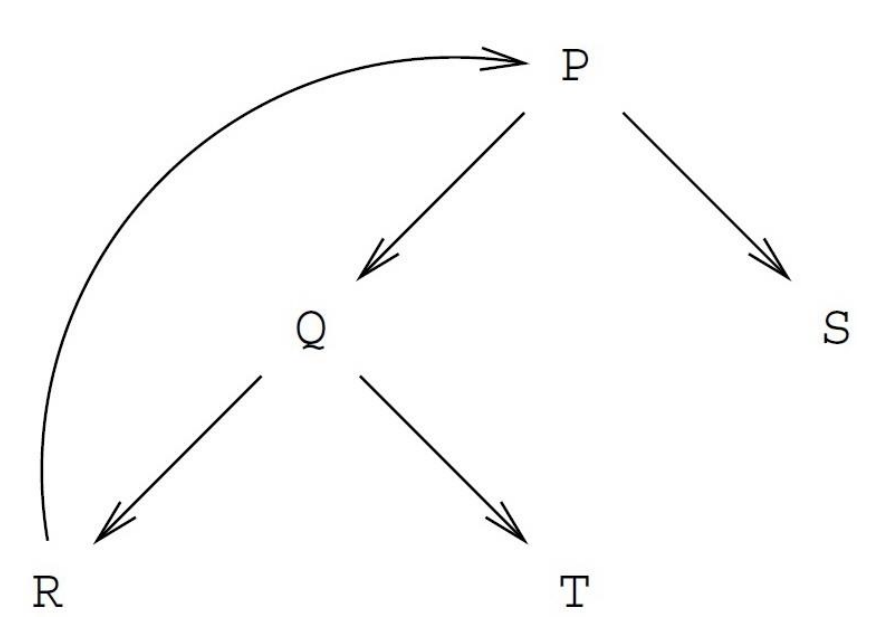
\includegraphics[width=0.5\linewidth]{images/calling-graph-1.png}
    \caption{An example of a calling graph.}%
    \label{fig:calling-graph-1}
\end{figure}

\begin{figure}[]
    \centering
    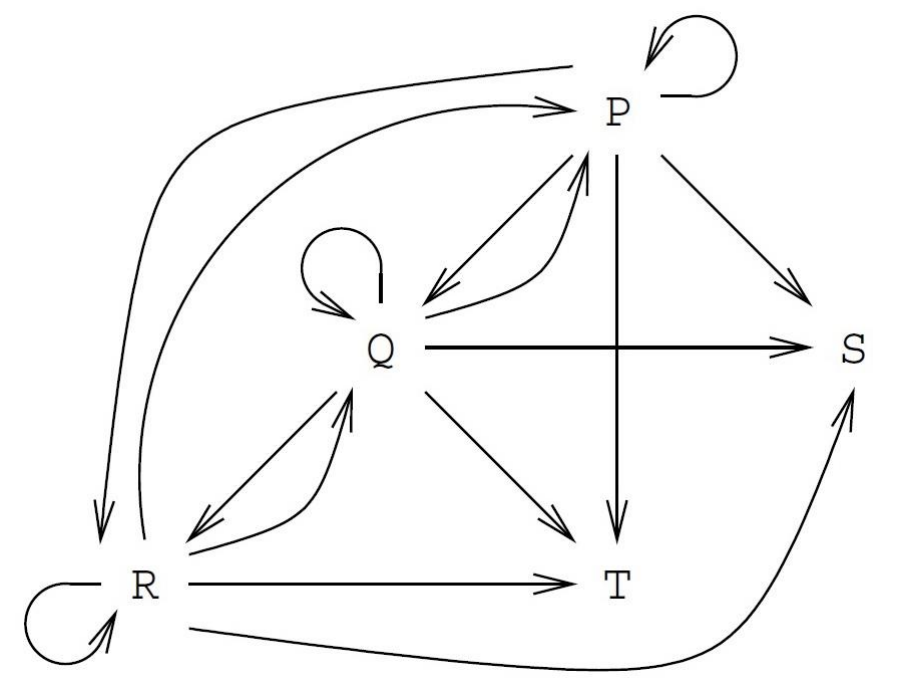
\includegraphics[width=0.5\linewidth]{images/calling-graph-2.png}
    \caption{An example of a transitive closure of a calling graph.}
    \label{fig:calling-graph-2}
\end{figure}

\begin{example}
    Consider the code below.
    \begin{center}
        \ttfamily
        \begin{tabular}{l}
            \toprule
            void P() \{ ... Q(); ... S(); ... \} \\
            void Q() \{ ... R(); ... T(); ... \} \\
            void R() \{ ... P(); ... \} \\
            void S() \{ ... \} \\
            void T() \{ ... \} \\
            \bottomrule
        \end{tabular}
    \end{center}
    We can draw an initial calling graph, as shown in Figure 
    \ref{fig:calling-graph-1}.
    As you can see though, \texttt{P()} will eventually call \texttt{R()}
    through \texttt{Q()}.
    We can produce the \textbf{transitive closure} of our initial calling graph,
    as shown in Figure \ref{fig:calling-graph-2}.
\end{example}

For a program with $n$ procedures, a recursive transitive closure algorithm
needs $O(n^3)$ time which is too much for practical applications;
however, in relatively \emph{sparse} programs it works in more like $O(n)$
time.

It is beneficially to avoid recursive definitions in regular expressions,
but how can we do this?

\begin{definition}[Regular definition]
    A \textbf{regular definition} is a sequence of definitions of the
    form
    \[ \{d_1 \to r_1, d_2 \to r_2, \ldots, d_k \to r_k\} \]
    where
    \begin{enumerate}
        \item each $d_i$ is distinct and $d_i \not \in \Sigma$; and
        \item each $r_i$ is a regular expression in 
            $\Sigma \cup \{r_1, r_2, \ldots, r_{i - 1}\}$.
    \end{enumerate}
\end{definition}

We avoid recursive definitions by sequentially \emph{eliminating} all $d_i$'s.
Therefoer, if we can write a set of regular expressions as a regular definition,
then we have no recursive definitions.
